\section{Automatisierte dynamische Softwaretests}

Zum Prüfen der Korrektheit seiner Arbeit macht jeder Programmierer mindestens manuelle Tests. Bei einer Webanwendung hieße dies konkret, den Webserver zu starten und mittels eines Browsers durch die Anwendung zu navigieren, Daten anzulegen und Ausgaben der Anwendung zu kontrollieren. Mit zunehmender Größe einer Anwendung wird es immer aufwändiger, die Software zu testen, da nach jedem Hinzufügen von Funktionalität eigentlich alle Aspekte wieder getestet werden müssen, um Regressionsfehler auszuschließen.

Stattdessen werden automatisierte Softwaretests instrumentalisiert, um auf Knopfdruck alle bisher programmierten Tests auszuführen und so ein Bild über den Zustand der Anwendung zu erhalten. So ist Automatisiertes Testen dem manuellem Testen, das auch Ad-Hoc-Testen genannt wird, in kürzester Zeit zeitlich überlegen \citep{rappin_rails_2011}.

Dynamische Testverfahren haben gemeinsam, dass sie stichpunktartig testen, damit die Korrektheit des Programmes nicht beweisen können und die Ausführung des Programmcodes mit konkreten Eingabewerten \cite{liggesmeyer_modultest_1990}[S. 49]. Diese Stichproben werden als \textbf{Testdaten} bezeichnet, die optimalierweise repräsentativ, fehlersensitiv, redundanzarm und ökonomisch sind \citep{liggesmeyer_modultest_1990}[S. 51].

Neben den dynamischen Tests, also Tests die Programmcode ausführen, gibt es statische Analyseverfahren, wie formale Verifikation, symbolische Testverfahren oder statische Analysen. Einige statische Anaylsen werden später im Abschnitt \ref{sec:metrics} vorgestellt. Andere statische Testverfahren sind nicht Gegenstand dieser Diplomarbeit.

\subsection{Motivation zm Anlegen von Tests}
Tests dienen in erster Linie dazu, das Vorhandensein bzw. Nichtvorhandensein von Software-Fehlern zu belegen \citep{goodliffe_code_2006}.

Getester Code gilt im Allgemeinen als robuster, korrekter und leichter zu warten \citep{rappin_rails_2011}. Im Umkehrschluss bedeutet dies, drastisch formuliert, dass ungetestete Software vorherbestimmt ist, Fehler zu haben \citep{goodliffe_code_2006}.

Die meisten Programmierer finden Testen besser als Debuggen. Testen führt zu einer Minimierung der Debugphase undmacht den Software Entwicklungsprozess für Programmierer attraktiver und für Projektleiter leichter zu planen \citep{orsini_rails_2007} und insgesamt preiswerter macht \citep{liggesmeyer_modultest_1990}[S.13].

%TODO Kent Beck?

\subsection{Arten von Tests}
Tests können nach verschiedenen Gesichtspunkten eingeteilt werden. In vielen konkreten Fällen reich eine eindimensionale Einordnung nicht aus, und Test können ebenso Teil von mehreren Kategorien sein.
\begin{figure}[hp]
 \centering
 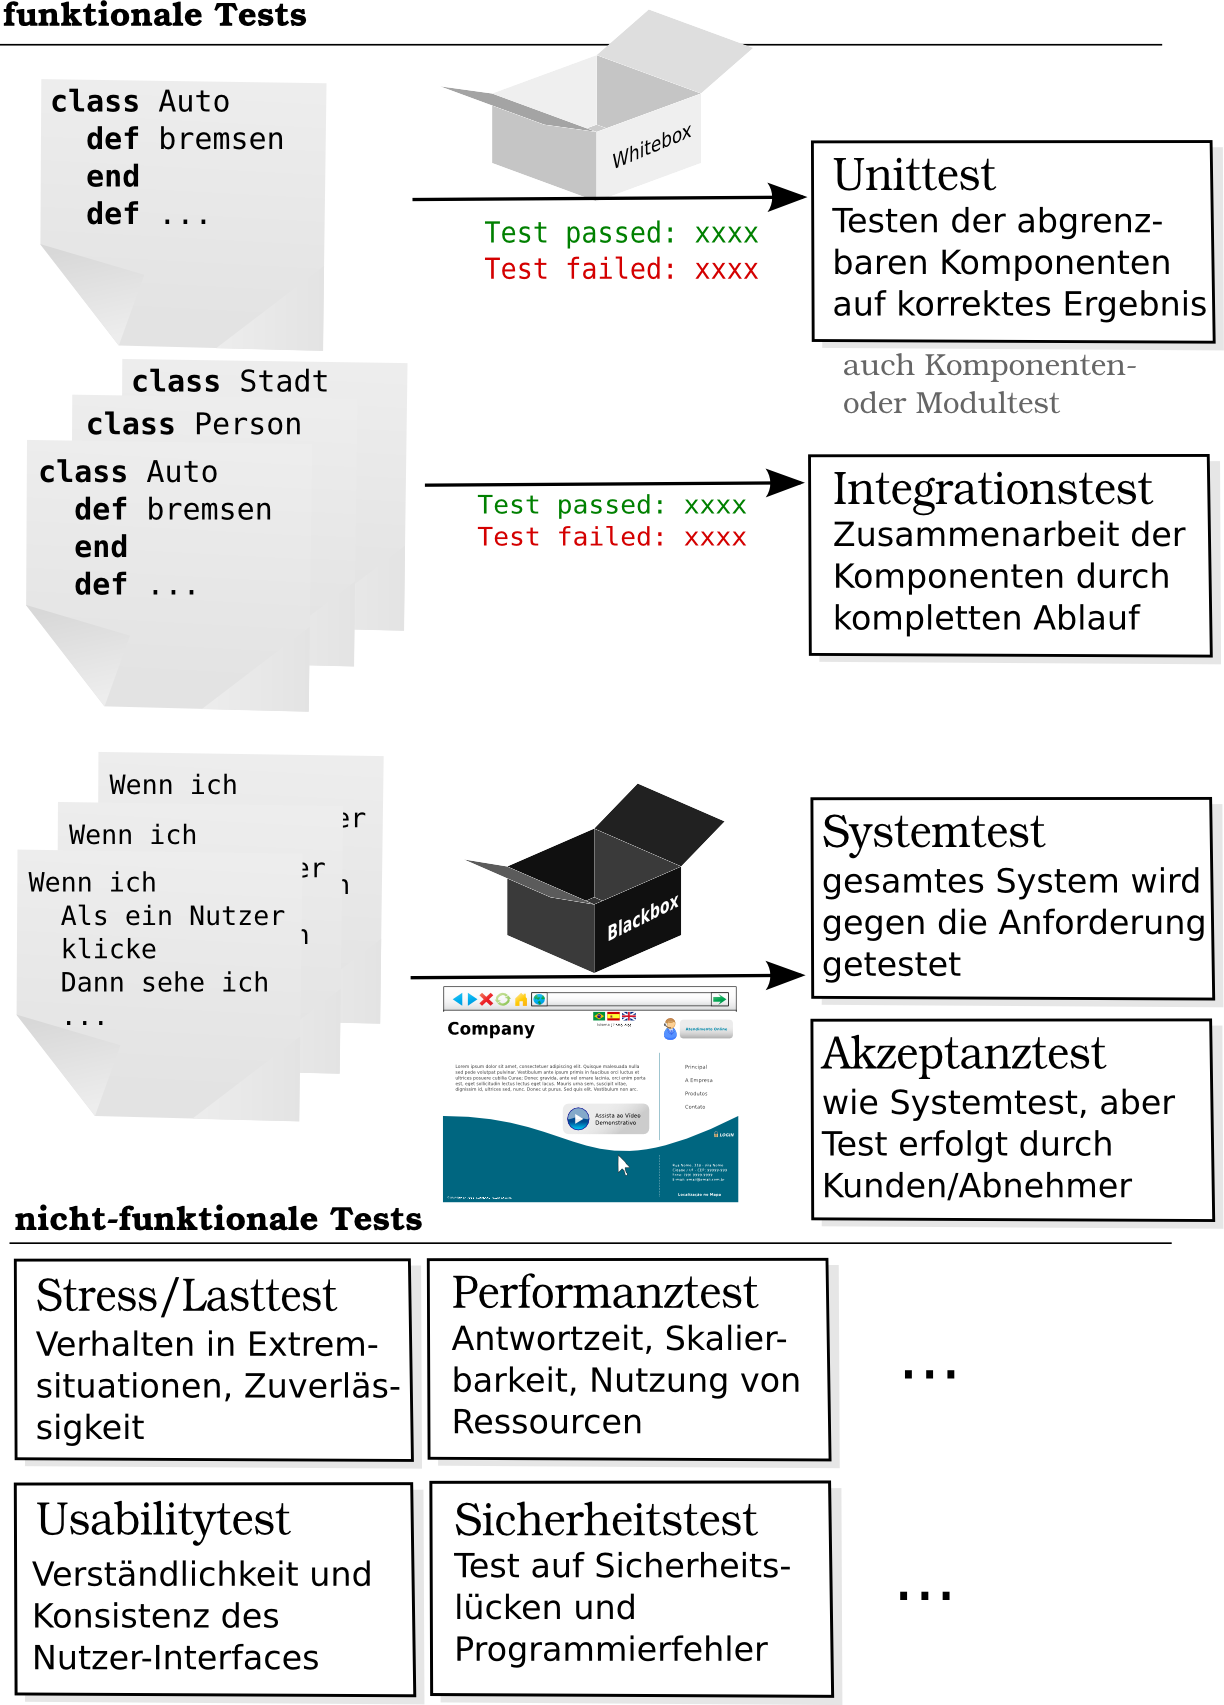
\includegraphics[width=\textwidth]{./diagrams/testarten.png}
 % testarten.pdf: 0x0 pixel, 300dpi, 0.00x0.00 cm, bb=
 \imgsource{Bildquelle: Der Author}
 \caption{Einteilung der Tests}
 \label{fig:testArten}
\end{figure}

\paragraph{Einteilung nach Sichtbarkeit des Quellcodes} Tests werden in \textbf{Whitebox} und \textbf{Blackbox}-Tests eingeteilt. 
Whitebox-Tests finden mit Wissen über den zugrundeliegenden Code statt. Ziel eines Whitebox-basierten Testverfahrens ist es, soviele Codeabschnitt wie möglich zu testen. Blackboxtests dagegen ignorieren den inneren Aufbau der Klassen und testen entweder nur Schnittstellen oder das Gesamtsystem, fokussieren also Aktionen und Rückmeldungen des Systems. Das Ziel eines Blackbox-basierten Tests, ist die Korrektheit der Software gegenüber den Spezifikationen.
Ein Spezialfall sind die sogenannten \textbf{Greybox}-Tests, die insbesondere bei der Testgetriebenen Entwicklung auftreten. Da der Test zuerst entwickelt wird, ist noch kein Wissen über den Zielquellcode vorhanden.

\paragraph{Einteilung nach Testziel} (nach \cite{hunt_pragmatic_1999}[S. 238ff])
\begin{description}
 \item[Unittests] Hierbei werden die Einheiten des Programmes auf ihr Verhalten getestet. Dies stellt die Basis für die meist darauffolgenden Integrationstests dar.
 \item[Integrationstests]  das Zusammenspiel zwischen Klassen wird getestet, welche ein gemeinsames Subsystem darstellen (Modul). Hier kann eine Bottom-Up oder Top-Down-Integrationsstrategie verfolgt werden,d.h. ob man mit denjenigen Modulen beginnt, die keine Abhängigkeiten haben und im Ableitungsbaum immer weiter nach oben integriert (bottom-up), oder mit dem zentralen Modul anfängt und nach und nach alle abhängigen oder abgeleiteten Module testet (Top-Down).
 \item[Validierung und Verifikation] Testet den Fortschritt der Anwendung in Bezug auf die funktionalen Anforderungen. Dies ist meist ein Blackboxtest und testet das System als ganzes (=Systemtest). Ein Spezialfall ist der Akzeptanztest. Hierbei nimmt der Kunde eine Anforderung/Feature ab.
 \item[Ressourcennutzung, Performanz, Verhalten im Fehlerfall] Die vorherigen Tests finden i.d.R. unter idealen Bedingungen statt. Diese Testkategorie versucht das Applikationsverhalten unter realen Bedingungen zu simulieren. Beim Verhalten im Fehlerfall soll getestet werden, dass der Nutzer nicht durch kryptische Fehlermeldungen verwirrt wird, oder z.B. sein Fortschritt gespeichert wurde. Last und Performanztests stellen sicher, dass die Anwendung eine große Zahl von Nutzern oder eine große Menge an Daten verarbeiten kann.
 \item[Usability Testing] Diese Testmethode kann gegenüber den bisher genannten nicht automatisiert werden, und benötigt immer einen zukünftigen Endanwender. Ziel ist es, die Benutzbarkeit und Handhabung zu testen. Dies wird durch Beobachtung von Kandidaten, meist in einer präperierten Umgebung (Usability Labor) geprüft.
\end{description}

\paragraph{Einteilung nach Testvollständigkeit} Tests können auch nach dem Gesichtspunkt eingeteilt werden, wie eine Testvollständigkeit beurteilt wird und notwendige Testfälle generiert werden \citep{liggesmeyer_modultest_1990}:
\begin{description}
 \item[Kontrollflussorientierter Test] betrachtet den Quelltext und leitet daraus notwendige Unittests ab
 \item[Datenflussorientierter Test] Beobachtet die Variablendefinitionen, Zugriffe und Entscheidungen anhand der Variablen
 \item[Funktionaler Test] leitet aus den funktionalen Spezifikationen Testfälle her
 \item[Diversifizierender Test] Testet verschiedene Versionen eines Programmes gegeneinander. Dies beinhaltet z.B. Mutationentest, der später im Abschnitt \ref{sec:mutation} \textit{\nameref{sec:mutation}} als Metrik zur Beurteilung der Tests erläutert wird.
\end{description}
\subsection{Unittest}
Da die \glossar{TDD} in ihrer Reinform auf dem Unittest basiert, soll diese Testgattung im Vorfeld etwas näher beleuchtet werden.

Ziel des Unittests ist es, frühzeitig Fehler im Code zu finden. Der Unit, oder Modultest beschreibt das Testen der Einheiten eines Programms, die im Sinne der Testung nicht weiter zerlegt werden können. Dies können die Funktionen, oder bei einer objektorientierten Sprache, die Klassen sein. Die Objekte unter Beobachtung (Objects under Test) werden beim Unittest werden in strenger Isolation zu den restlichen Units ausgeführt. Abhängigkeiten der Module untereinander und von unterlagerten Diensten werden durch \glossarpl{Test-Double} simuliert. Dies ist notwendig um sicherzustellen, dass gefundende Fehler von dem betreffendem Modul verursacht wurden, und nicht durch äußere Einflüsse. Diese Isolierung macht das Testen einfacher \citep{goodliffe_code_2006}.



Unittests werden fast immer automatisiert ausgeführt. Verwendung finden dabei meist immer sogenannte Test-Frameworks. Eine der meist-verbreitetsten sind die Frameworks auf Basis von xUnit, die in nahezu allen (objektorientierten) Sprachen Vertreter haben, so z.B. Test::Unit/MiniTest in Ruby, JUnit in Java oder NUnit in C\#.

Ein solcher Test besteht in der Regel aus 4 Teilen:
\begin{enumerate}
 \item Initialisierung der Test-Umgebung und der Objekte
 \item Ausführung der zu testenden Aktion, die den Systemzustand ändert
 \item Prüfen der spezifizierten Erwartungen (Assertions)
 \item Aufräumen nicht mehr benötigter Objekte, File-Pointer, Sockets, Leeren der Datenbank u.ä 
\end{enumerate}

\paragraph{Komponententest}
Ziel des Komponententest ist es, verschiedene Units in Kombination als eine vollständige Komponente zu testen \citep{goodliffe_code_2006}.

 \subsection{Test Doubles -- Mocks und Stubs}
  \label{sec:mocks}
  Beim isolierte Testen wird durch Abhängigkeiten aller Art erschwert. Dies können z.B. Klassen sein, die noch nicht implementiert wurden, externe Ressourcen (Netzwerkzugriffe, Versenden von Mails) oder externe unterliegende Prozesse (Bezahlen in einem Onlineshop, Datenbanken) sein. In diesen Situationen ist es angebracht, auf sogenannte Test-Doubles, meist Mocks und Stubs, zurückzugreifen.
  
  Ein \textbf{Stub} ist eine nachahmende Funktion oder Objekt, welches die schwer zu isolierende Klasse während des Testfalls ersetzt. Im Beispiel ein Bezahlprozess einer Bestellung.
  \begin{lstlisting}
def test_report_failed_payment
  Payment.stubs(:pay).returns(false)
  
  bestellung = Bestellung.new()
  bestellung.commit()
  
  assert bestellung.not_valid?
end
  \end{lstlisting}
  Mit dem oben angegeben (Pseudo-) Rubycode würde man z.B. mittels des Mock-Frameworks "`mocha"`\footnote{\url{http://mocha.rubyforge.org/}} ein Stubobjekt erzeugen, welches den Bezahlprozess nachahmt, und die Methode "`pay"' ersetzt, so dass sie immer "`false"' zurückgibt, d.h. der extern Bezahlvorgang wird in diesem Test fehlschlagen, z.B. wenn der Benutzer falsche Zahlungsdaten angegeben hat. Auf diese Weise könne komplexe Operationen auf ihre Interfaces reduziert werden. Außerdem machen Stubs den Test i.d.R. schneller, da statt der potentiell komplexen und langsamen Operationen statische Werte geliefert werden.
  
  
  Als Ergänzung dazu gibt es \textbf{Mocks}. Ähnlich wie die Stubs ersetzen sie Methoden oder Objekte, um statt komplexer Operationen fixe Werte zurückzugeben. Zusätzlich dienen Mocks selbst als Testfall. Ein Mock wartet darauf, ob die Methode, wie sie definiert wurde, auch tatsächlich aufgerufen wurde.
  
  Hier z.B. ein Mock um einen Netzwerkzugriff zu testen und abzufangen.
  \begin{lstlisting}
def test_always_fail
  HTTP.expects(:get).with("http://www.google.com")
end
  \end{lstlisting}
  Der gezeigte Test wird immer fehlschlagen, da von einem Mock erwartet wird, dass die nachgeahmte Funktion während des Tests genau einmal aufgerufen wird. Ist dies nicht der Fall, gilt der Test als nicht bestanden. Mocks fungieren somit als zusätzliche Möglichkeit Interna des Programmflusses zu testen. 

\subsection{System- und Akzeptanztests}

Der Unittest ist als Whitebox-Test auf Wissen über den Quelltext angewiesen, und der Zweck ist es, Fehlerfreiheit zu gewähren. Der \textbf{Systemtest} dagegen testet das gesamte integrierte System, meist aus der Sicht eines Anwenders, mit dem Ziel, die Software gegenüber den Anforderungen zu validieren. Diese Tests finden unter realen Bedingungen mit realen Daten statt und untersucht, meist sogar auf einer den Parametern der Produktionsumgebung nahe-kommende Hard- und Softwareumgebung.

Der \textbf{Akzeptanztest} ist ein Spezialfall des Systemtests. Hier führt der Auftraggeber der Software den Test selbst durch. Er nutzt den Akzeptanztest, um zu entscheiden, ob er die Software akzeptiert, woher der Name rührt.
Innerhalb des Kontextes der Agilen Programmierung, dem auch die Testgetriebene Software zuzurechnen ist, dienen Akzeptanztests, um den Fortschritt bei der Bearbeitung der "`Geschichten"' (user stories) zu überwachen.

Für das Testen von Webserveranwendungen spielt die Simulation eines Browsers eine große Rolle, um die Tests unter möglichst realen Bedingungen durchzuführen. Hierbei bedient man sich der Fernsteuerung eines Browsern mittels einer Middleware, die es ermöglicht innerhalb eines Testfalls einen Webbrowser zu starten. Eine der bekanntesten dieser Middlewares ist das Framework \textbf{Selenium}\footnote{\url{http://seleniumhq.org/}}, welches Firefox, Internet Explorer und Google Chrome fernsteuern kann. Dies ermöglicht eine sehr detaillierte Testung auf Browserinkompatibilitäten, da es unter den Browsern gewisse Unterschiede in der Ausführung von Javascript und Darstellung von Elementen gibt. Dieses Tool wird u.a. von Google, Oracle und eBay zum Tests ihrer Anwendungen verwendet und weiterentwickelt \citep{selenium_hq_selenium_2010}.
